\documentclass[11pt,a4paper,roman,unicode]{moderncv}
\PassOptionsToPackage{
  pdfpagelabels=false,
  urlcolor=magenta,
  colorlinks=True,
  citecolor=gray}{hyperref} 

% fonts
\usepackage{mathpazo}
%% % URls
%% \usepackage{hyperref}
%% \hypersetup{
%%   colorlinks=true,
%%   citecolor=gray,
%%   urlcolor=magenta, %couleur des hyperliens
%% }

\moderncvtheme[blue]{classic}                
\usepackage[utf8]{inputenc}
\usepackage[top=1.1cm, bottom=1.1cm, left=2cm, right=2cm]{geometry}
%\usepackage[scale=0.8]{geometry}

\setlength{\hintscolumnwidth}{3.8cm}
\setlength{\makecvtitlenamewidth}{12cm}
\renewcommand*{\namefont}{\fontsize{24}{29}\mdseries\upshape}

\firstname{Isaac}
\familyname{Kamga}
\title{M.Sc. Graduate}   
\email{u2isaac@gmail.com}                      
\photo[64pt]{Candle}
\address{GDG Buea, Cameroon.}
%\mobile{<Tel portable>}                    
\homepage{https://github.com/Izakey}

\begin{document}
\maketitle

\section{Education}
\begin{figure}[htbp]
\centering
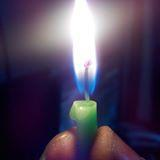
\includegraphics[trim=1cm 2cm 3cm 4cm, clip=true, totalheight=0.5\textheight]{Candle.png}
\caption[Candle]{Candle}
\label{Candle}
\end{figure}

\cventry{2010 -- 2011}{MSc. Cryptology and Information Security}{University of Bordeaux
1}{}{}{Pentesting for telecom and VoIP-like protocols including SS7, SIGTRAN, SIP, GTP}
\cventry{2009 -- 2010}{Maîtrise ès Mathématiques}{University of Bordeaux 1}{}{}
{On explicit constructions of ``good'' LDPC QECCs (\emph{Low-Density Parity-Check Quantum Error-Correcting Codes}). Supervised by Gilles ZEMOR}
\cventry{2005 -- 2008}{BSc. Mathematics and Computer Science}{University of Buea}{}{}
{}

\section{Professional Experience}
\cventry{\llap{Oct 2012 -- Oct 2014}}{Research engineer}{PARIETAL -- INRIA, Neurospin CEA, Saclay}{}{}{
Non-smooth convex optimization; preprocessing and statistical analysis of fMRI data; registration algorithms;
machine learning on fMRI data; software engineering\newline{}}
\cventry{Sep 2011 -- Oct 2012}{Freelancer and Open-Source}{Various employers}{}{}{
Simulations for CR (Cognitive Radio) research; Windows system programming (DLLs, user-space
root-kits, etc.); implementation of Machine Learning algorithms\newline{}}

\cventry{Mar 2011 -- Aug 2011}{Cryptology and Security intern}{P1 Security}{Paris}{France}{
Implementation of an event-driven pentesting framework for telecom and VoIP-like protocols
\newline{}}

\section{IT and Computing Skills}
%\footnotesize{\emph{Software I have developed or contributed to can be found at https://github.com/dohmatob}}
\cvitem{\llap{Programming Languages}}{Python, ASM x86, C/C++, MATLAB, R, PARI/GP, Emacs-Lisp, javascript}
\cvitem{Maching Learning}{LibSVM, scikit-learn, pandas}
\cvitem{Neuro-imaging}{nilearn, SPM, FSL, nipy, nipype, freesurfer, mayavi, pypreprocess}
\cvitem{Software Engineering}{OOP, TDD, EDD, version control (git, github), continuous integration (travis), parallel computing}
\cvitem{Operating Systems}{Linux, Windows (including shell scripting and system programming skills)}
%% \cvitem{Network Protocols}{TCP/IP, SMB, IPSec, LDAP, SSL, SIP, DNS}
%% \cvitem{Cryptology}{Number Theory, Elliptic Curves, Smart Cards, Asymmetric Cryptography (RSA), Symmetric
%% Cryptography (PKI, DH, DES, AES)}
%% \cvitem{Security tools}{Snort, Wireshark, Nmap, METASPLOIT, OllyDbg, Immunity Debugger, IDA Pro, SPIKE}
\cvitem{My github profile}{\url{https://github.com/dohmatob}}

\section{Scientific Publications (see complete google scholar)}
\cvitem{2014}{\begin{itemize}
  \item{A. ABRAHAM, E. DOHMATOB, B. THIRION, D. SAMARAS, G. VAROQUAUX,
``\emph{Region segmentation for sparse decompositions: better brain parcellations from rest fMRI}''.
\url{http://stmi2014.ece.cornell.edu/papers/STMI-P-9.pdf}}
  \item{B. THIRION, G. Varoquaux, E. DOHMATOB, J.-B. POLINE,
``\emph{Which fMRI clustering gives good brain parcellations?}''.
Frontiers in Neuroinformatics. \url{http://journal.frontiersin.org/Journal/10.3389/fnins.2014.00167/abstract}}
  \item{E. DOHMATOB, A. Gramfort, B. THIRION, G. Varoquaux
    ``\emph{Benchmarking solvers for TV-$\ell_{1}$  least-squares and logistic regression in brain imaging}''.
    Pattern Recoginition in Neuroimaging (PRNI), \emph{IEEE}. \url{http://hal.inria.fr/hal-00991743}}
\end{itemize}}
\cvitem{2013}{
\begin{itemize}
\item{A. ABRAHAM, E. DOHMATOB, B. THIRION, D. SAMARAS, and G. VAROQUAUX,
  ``\emph{Extracting brain regions from rest fMRI with Total-Variation constrained dictionary learning}''.
  MICCAI - 16th International Conference on Medical Image Computing and Computer Assisted Intervention - 2013 (2013).
  \url{http://hal.inria.fr/hal-00853242}}
\end{itemize}
}

\section{Contributions to open-source software projects}
\cvitem{Neuro-Imaging}{nipy \url{http://nipy.org}, nilearn \url{http://nilearn.github.io},
  pypreprocess \url{https://github.com/neurospin/pypreprocess}}
\cvitem{Personal projects}{See complete list on my github profile: \url{https://github.com/dohmatob}}
%% \cvitem{My \emph{Open Source Report Card}}{Tentatively, an impartial automatically generated statistical summary of
%% my ``contributions heat map'' can be found at \url{http://osrc.dfm.io/dohmatob/}}
\section{Scientific Talks}
\cvitem{PRNI 2014}{At the PRNI (Pattern Recoginition in Neuroimaging) conference that took place
3rd -- 6th June 2014 (Max-Planck Institute for Intelligent Systems, Tuebingen -- Germany), I presented my work,
``\emph{Benchmarking solvers for TV-$\ell_{1}$ least-squares and logistic regression in brain imaging}''
(\url{http://hal.inria.fr/hal-00991743})%% , under the ``Advances in fMRI analysis'' section of the conference
  .}
\cvitem{Forum STIC 2014}{Poster presentation for PRNI2014 paper at STIC,
Paris-Saclay, France.}

\cvitem{OHBM 2015}{Oral + poster presentation on\textit{``SpaceNet:
Multivariate brain decoding and segmentation''},  Honolulu, Hawaii, USA}

\cvitem{PRNI 2015}{Oral presentation on\textit{``Speeding-up
model selection in GraphNet via early-stopping and
feature-screening''}, Stanfod, USA}

\section{Hackathon Experience}
%% \cvitem{\llap{Parietal retreat,}\\ 6th -- 8th April 2014}{Virgile FRITSCH and I did VBM (Voxel-Based Morphometry) on a public dataset (Oasis database). The outcome of this
%% sprint is summarized here \url{https://github.com/Parietal-INRIA/parietal-python/wiki/VBM-dataset-for-nilearn}}
\cvitem{\llap{Google Hash Code Paris, }\\ 2014}{Implementation of
  street-viewer for Paris. Problem can be modelled as a TSP.}
\cvitem{\llap{Brainhack Paris,}\\ 23rd -- 26th Oct 2013}{Group
  analysis on Henson's multi-modal faces vs objects dataset.}

\section{Languages}
\cvline{Bilingual}{English (fluent), French (fluent)}

\section{Awards and Scholarships}
\cvitem{2014}{Honourable Mention (2nd price) awarded to the paper ``\emph{Benchmarking solvers for
TV-$\ell_{1}$ least-squares and logistic regression in brain imaging}'', by E. DOHMATOB, A. GRAMFORT,
B. THIRION, G. VAROQUAUX (\url{http://hal.inria.fr/hal-00991743}), presented at the 4th international
workshop on Pattern Recognition in NeuroImaging (PRNI 2014), Max-Planck Institute for Intelligent Systems,
Tuebingen -- Germany}
\cvitem{2009 - 2011}{Erasmus Mundus, ALGANT, University of Bordeaux 1}

\section{Interests}
\cvline{Research}{convex optimization, nonlinear registration, machine
learning, human connectome mapping, game theory}
\cvline{Hobbies}{Reading, dancing, running}

\end{document}
